\section{User Activity Inference Through EEG Data}
\label{sec:inference}

What information can be reflected from the EEG data remains to be an active research topic. Besides the traditional information such as the focal brain diagnosis, attention level, and meditation level, as we mentioned earlier, current research shows that EEG can possibly be used to predict viewed images~\cite{mindreading2017}, recognize individuals~\cite{chu2017individual}, transfer brain waves to texts~\cite{zhang2017converting}, monitor sleep~\cite{nakamura2017automatic},  and reveal personal information~\cite{martinovic2012feasibility}. However, the EEG data used in these research projects were collected by strict medical-use or research-use EEG devices. Whether the reduced-featured EEG data collected by home-use EEG IoT devices also have the potential to reveal user's activities remains unexplored. In this section, we present our deep learning model which can infer a user's current focusing activities with a high accuracy. As one can see, EEG data reflects rich information about a person's health condition; therefore, leakage of the personal EEG data is a severe violation of privacy.

\subsection{Overview}
Inspired by Zhang \emph{et al.}'s work~\cite{zhang2017converting,hochreiter1997long}, we leveraged the idea of parallel feature learning and built our own RCNN to classify user's focusing activities. RCNN is composed of a recurrent neural network (RNN) and a convolutional neural network (CNN). The reason for using RNN is because it is able to learn temporal features and EEG data is temporally correlated; and the reason for adopting CNN is because it is capable of learning the potential spatial features and EEG data is spatially correlated as well. Finally, we flattened all the features output by the CNN and RNN networks, concatenated them with several layers of fully connected feedforward neural networks to output the final predictions. The overall structure of the neural network is shown in Figure~\ref{fig:rcnn}. In order to identify a proper structure for our problem, we tested different numbers of layers for both RNN and CNN, from 3 layers to 8 layers; it turned out that a 5-layer structure for both RNN and CNN is the most effective because the in-sample accuracy of our training data increases most rapidly in this structure among all others. Note that we cannot directly apply Zhang \emph{et al.}'s work to our case because: (1) the size of the input features of their model is much higher than that of ours since they used BCI2000 data, (2) the prediction classifications are totally different, and (3) their model contains an autoencoder and an autodecoder which fit for more complicated situations. %This implies that directly applying Zhang's model does not pose meaningful sense.
In the following two subsections we detail the RNN and CNN structures. 

\begin{figure*}[t]
        \centering
        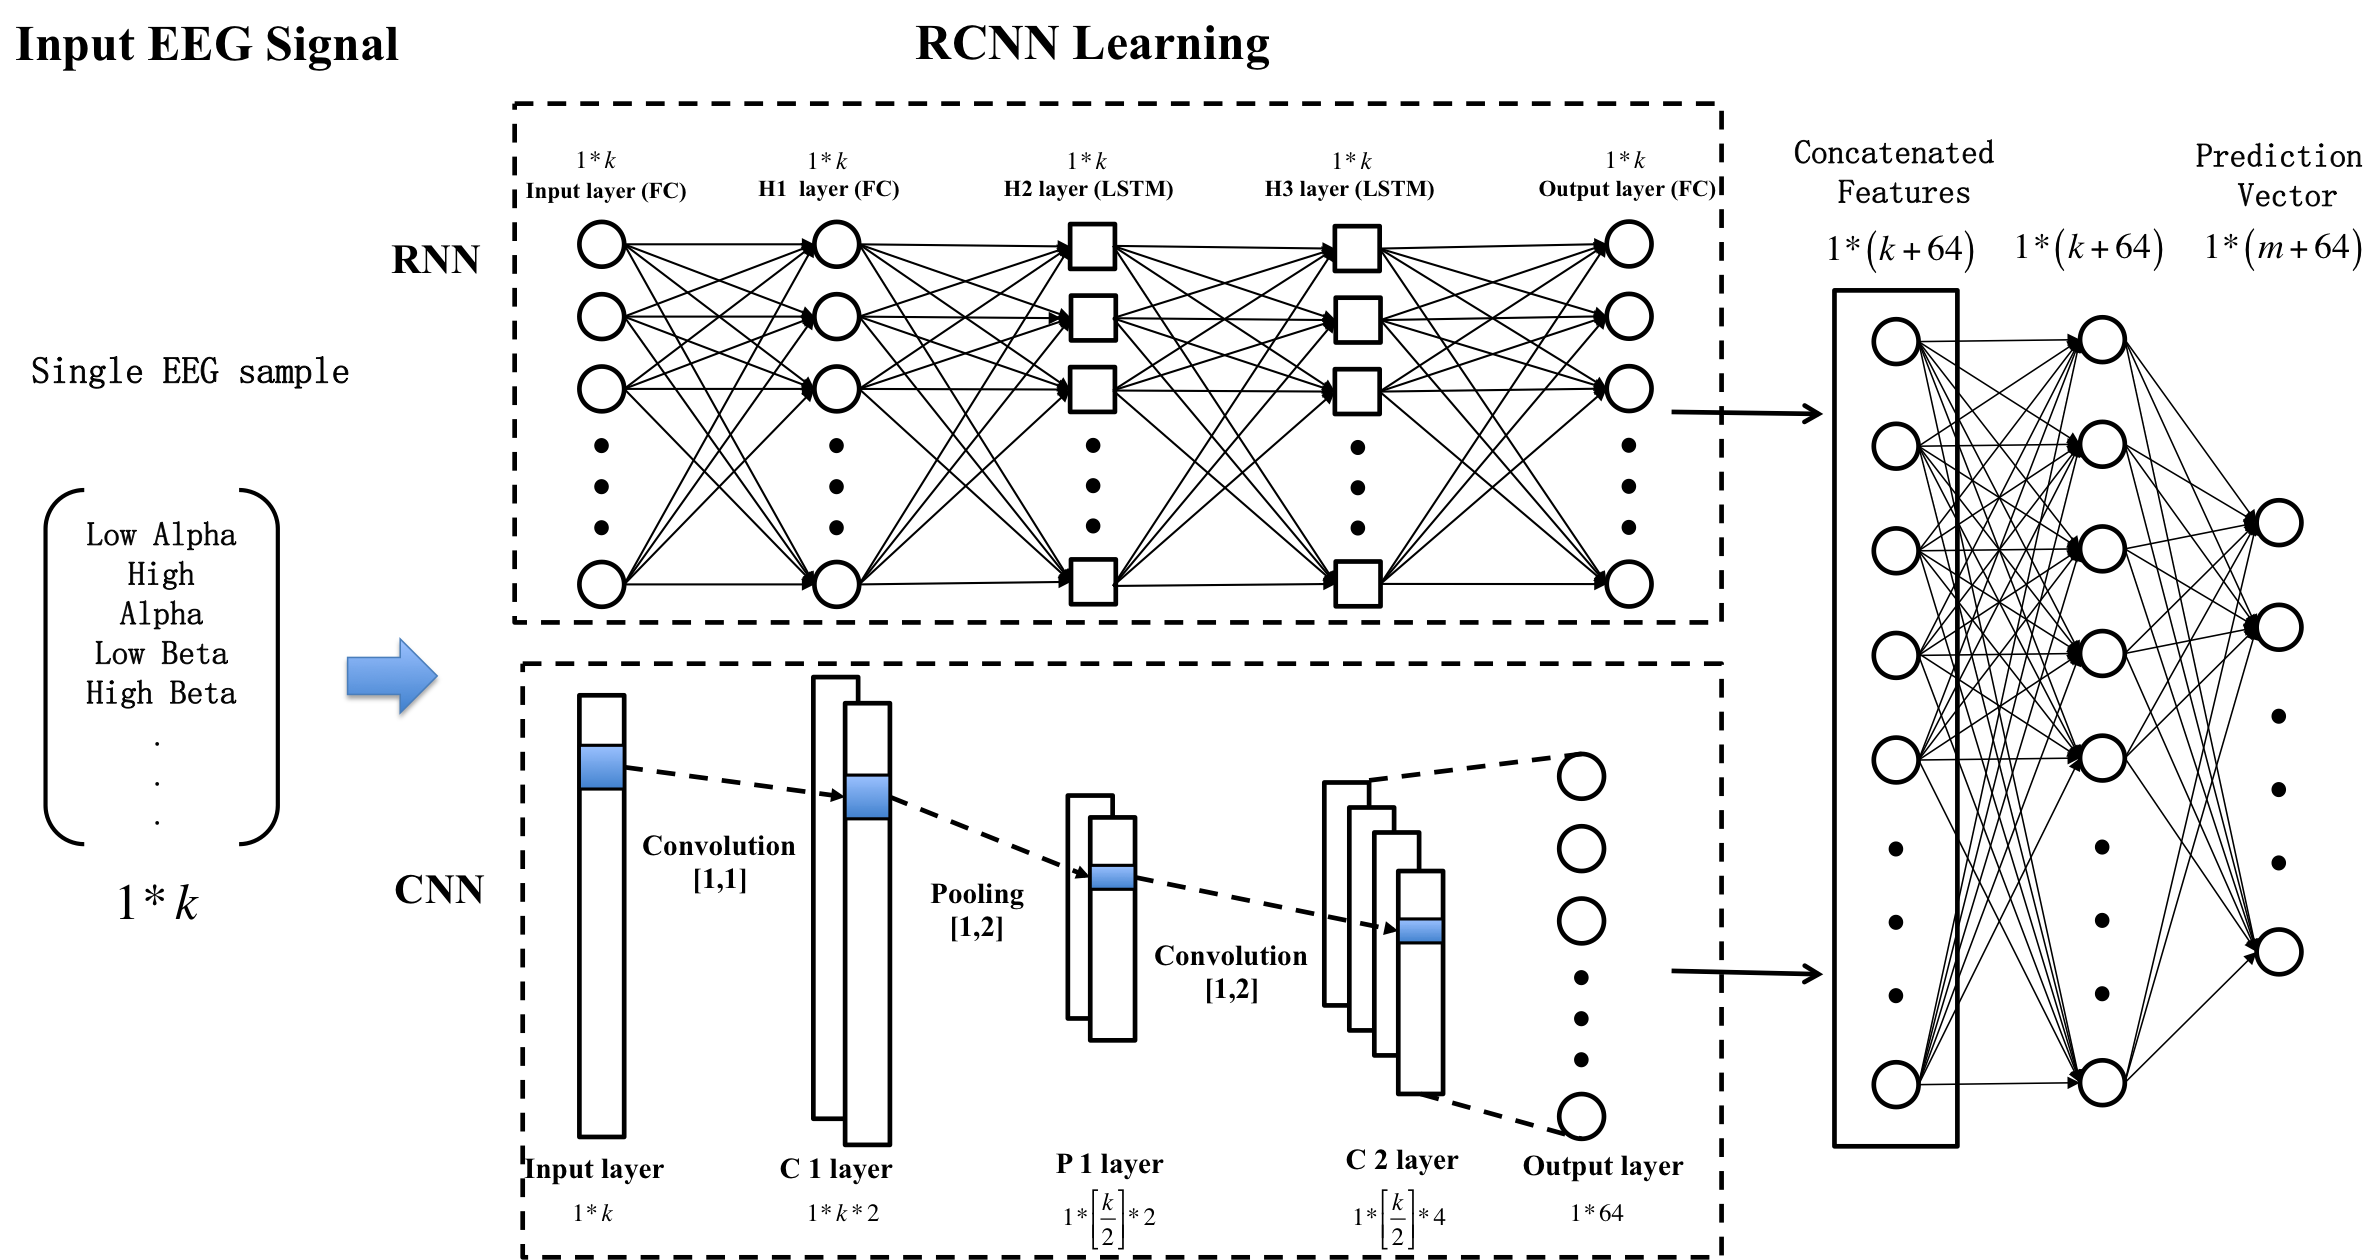
\includegraphics[width=\linewidth]{RCNN.png}
        \caption{The RCNN structure. There are 5 layers in the RNN model and 5 layers in the CNN model. The features output by RNN and CNN are concatenated by 3 fully connected layers for the final predictions.}
        \label{fig:rcnn}
\end{figure*}

\subsection{RNN Learning}
Our RNN has 5 layers in total: one fully connected feedforward layer as the input layer, three hidden layers which contain one layer of feedforward network and two layers of Long Short-Term Memory (LSTM) cells, and one fully connected feedforward layer as the output layer. Each layer contains $k$ neurons/cells where $k$ is the number of features of the EEG data. In our RNN model, EEG data is first resized into a 2-D vector with a shape of $[n,k]$, where $n$ is the number of samples, or batch size, before the data is fed into the network. For better elaboration, we employ $n=1$ meaning that only one sample of the features is fed into the network, to present the basic idea. Suppose we denote the data output by the $i$-th layer of our RNN model to be $X_i^{r}$, where $i=1,2,\cdots,5$, the weight vector between the $i$-th layer and the $i+1$-th layer to be $W_{i,i+1}^{r}$, and the bias vector of the $i$-th layer to be $B_{i}^{r}$. Having presented these notations, we can represent the relationship between the data from two neighboring layers in our model as:
\begin{equation}
X_{i+1}^{r} = \max(0, X_i^{r}* W_{i,i+1}^{r} + B_{i}^{r})
\end{equation} 
where $\max(0,x)$ is the rectifier linear unit (ReLU) used for the activation function. Having had a big picture of our RNN structure, our next step is to take a closer look at each LSTM cell. Suppose at time $t$, we denote $x_{t}$ to be a scalar data fed into a LSTM cell, $h_{t}$ to be the output data by the cell, $f_{I}$ to be the input gate, $f_F$ to be the forget gate, $f_O$ to be the output gate, and $C_{t}$ to be the cell state. Within a LSTM cell, the following calculations are performed:
\begin{gather}
f_{I} = \sigma (W_{I}\cdot h_{t-1} + W_{I} \cdot x_{t}) + B_{I}\\
\widetilde{C}_{t} = \tanh(W_{C}\cdot h_{t-1} + W_{C} \cdot x_{t} + B_{C})\\
f_{F} = \sigma (W_{F}\cdot h_{t-1} + W_{F} \cdot x_{t}) + B_{F}\\
C_{t} = f_{f} * C_{t-1} + f_{i} * \widetilde{C}_{t}\\
f_{O} = \sigma (W_{O}\cdot h_{t-1} + W_{O} \cdot x_{t}) + B_{O}\\
h_{t} = f_{o} * \tanh(C_{t})
\end{gather} 
where $\widetilde{C}_{t}$ is an intermediate value between $C_{t}$ and $C_{t-1}$, the variables with letters $W$ and $B$ refer to the weights and biases, respectively, for that specific gate or cell state, and $\sigma$ represents the sigmoid function which has the form of
\begin{equation}
\sigma(x) = \frac{1}{1+e^{-x}} = \frac{e^{x}}{e^{x} + 1}
\end{equation}
At last, our RNN outputs the features with the shape $[1, k]$. 

\subsection{CNN Learning}
Our CNN has 5 layers as well: one convolutional layer as the input layer, a max pooling layer, two convolutional layers, and one fully connected feedforward layer as the output layer. We denote the data output by the $i$-th layer to be $X_i^{c}$, where $i=1,2,\cdots,5$, the weight vector between the $i$-th layer and the $i+1$-th layer to be $W_{i,i+1}^{c}$, and the bias vector of the $i$-th layer to be $B_{i}^{c}$. Similar to RNN, EEG data is first resized into a 2-D vector with the shape of $[n,k]$. In the first convolutional layer, we set the filter with a size of $[1, 1]$ with zero-padding and output one more dimension in depth. Therefore, $X_1^{c}$ has the shape of $[1, k, 2]$. For the max pooling layer, we set the stride to be the shape of $[1, 2]$; therefore, $X_{2}^{c}$ has the shape of $[1, \ceil{k/2}, 2]$. We then set the filters for the following two convolutional layers to be $[1, 2]$ and $[1, 4]$, which yield the shapes of $X_3^{c}$ and $X_4^{c}$ to be $[1, \ceil{k/2}, 4]$ and $[1, \ceil{k/2}, 4]$, respectively. Then we flatten $X_4^{c}$ to feed into the last fully connected feedforward layer which outputs the features with a shape of $[1, 64]$. All layers use the ReLU as the activation function.

\subsection{Concatenation Layers}
Finally, we need to concatenate the features output by RNN and CNN to generate predictions. Our RNN model outputs features with a shape of $[1, k]$ and the CNN outputs features with a shape of $[1, 64]$. We simply concatenate the features to get the shape of $[1, k + 64]$ and feed them to two fully connected feedforward layers which output the features with shapes of $[1, k+64]$ and $[1, m]$, where $m$ is the number of classes of the user's activities. Both layers use ReLU as the activation function. Lastly, we use the Adam optimization algorithm~\cite{kingma2014adam} to reduce our loss function constructed by the softmax cross entropy shown below:
\begin{equation}
loss = - \sum_{j=1}^{m} y'_j \cdot \log(\frac{e^{y_j}}{\sum_{l=1}^m e^{y_l}})
\end{equation}
where $y_j$ is the predicted probability for the $j$-th class and $y'_j$ is the ground-truth probability for the $j$-th class.



